In this section, we test our WHVI implementation, specifically the inference and predictive quality of Bayesian deep neural networks that use WHVI linear layers.
We first focus on the toy example from Section 3.1 and then discuss regression experiments from Section 3.2 of the original paper.
% Some discrepancies on the toy example are already large enough that more complex experimentation is not meaningful.

\subsection{Toy example}\label{subsec:toy-example}
We consider the toy example from Section 3.1 in the original paper.
The authors do not provide an explicit formula for the function.
To replicate the experiment as closely as possible, we look at the plot and roughly observe some $(x, y)$ pairs -- extrema and in-between values.
We then use polynomial interpolation with a Vandermonde matrix to obtain a similar-looking function.
This function is visualized in Figure~\ref{fig:toy-function}.

\begin{figure}[h]
    \centering
    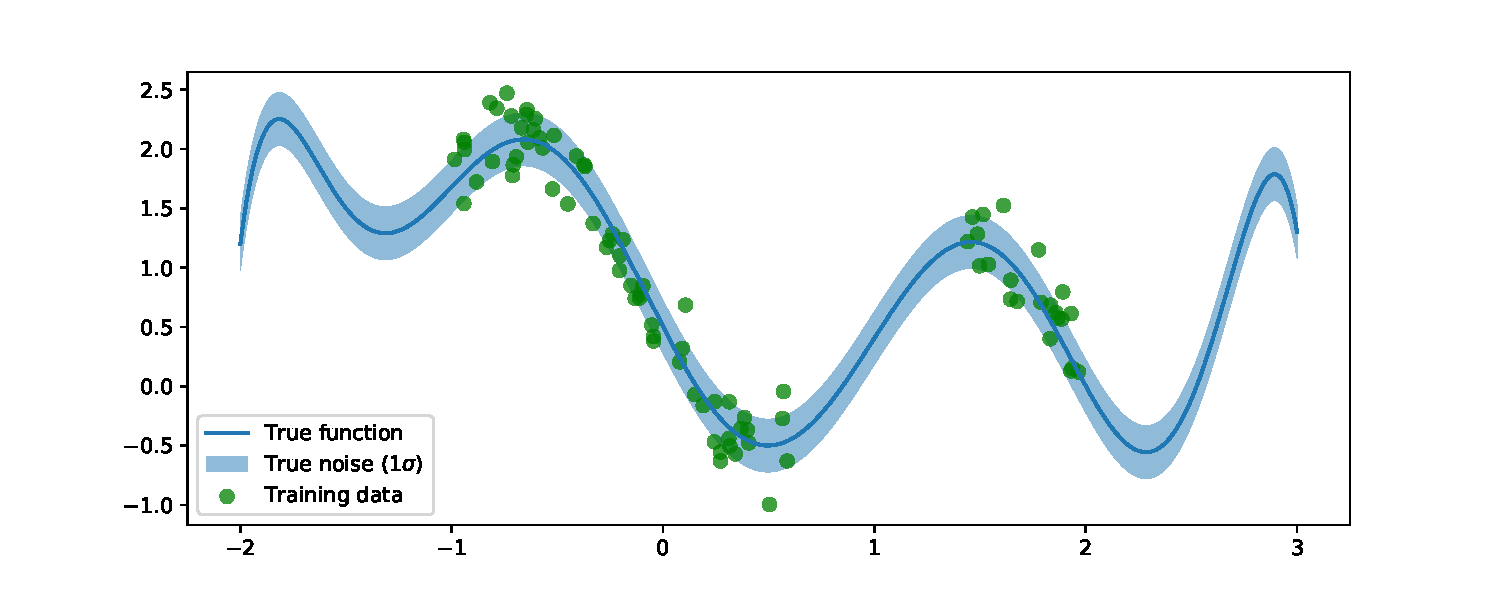
\includegraphics[width=1.0\hsize]{img/toy-function}
    \caption{Polynomial approximation to the toy function in the original paper.
    The exact form of this function up to two decimals is $f(x) = 0.50 -3.45x + 1.14x^2 + 4.36x^3 -0.93x^4 -1.77x^5 + 0.39x^6 + 0.22x^7 -0.06x^8$.
    The noise is normally distributed with $\sigma = \sqrt{\exp (-3)}$.
    }
    \label{fig:toy-function}
\end{figure}

The cosine activation function is no longer suitable given this different form of the function.
We check this by training a non-Bayesian model, which has the exact same architecture as the WHVI one (two hidden layers with 128 hidden units).
We found that the sigmoid activation performs slightly better and decided to use it in the WHVI experiment instead.
A comparison of the two non-Bayesian models with different activations can be seen in Figure~\ref{fig:toy-function-non-bayesian}.

\begin{figure}
    \centering
    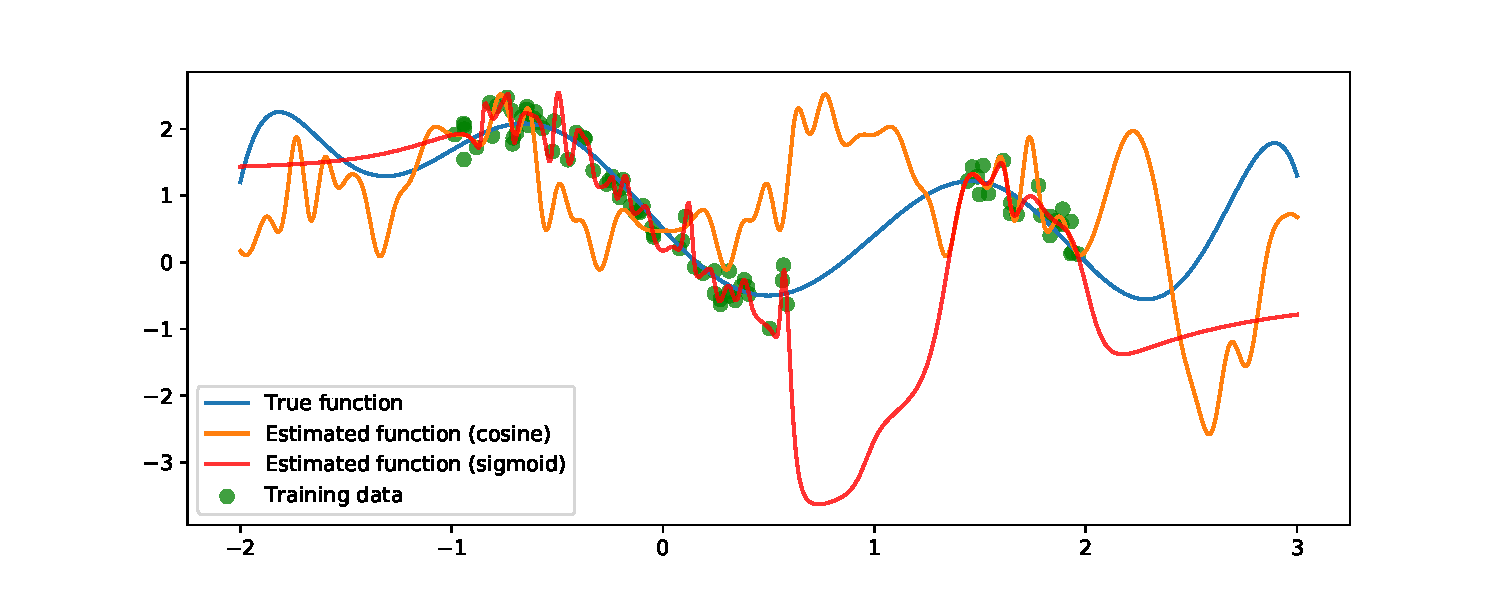
\includegraphics[width=1.0\hsize]{img/toy-function-non-bayesian}
    \caption{Comparison of the cosine and the sigmoid activation in a non-bayesian network.
    We decided to use sigmoid instead of cosine, because it seemed to capture the function more nicely on the left chunk of the data.}
    \label{fig:toy-function-non-bayesian}
\end{figure}

We trained the model with WHVI layers and found that the results depend heavily on initial $\lambda$ values in each layer as well as the initial scale $\sigma_0$ of the Gaussian likelihood.
The result is visualized in Figure~\ref{fig:toy-function-whvi}.
\begin{figure}[htbp]
    \centering
    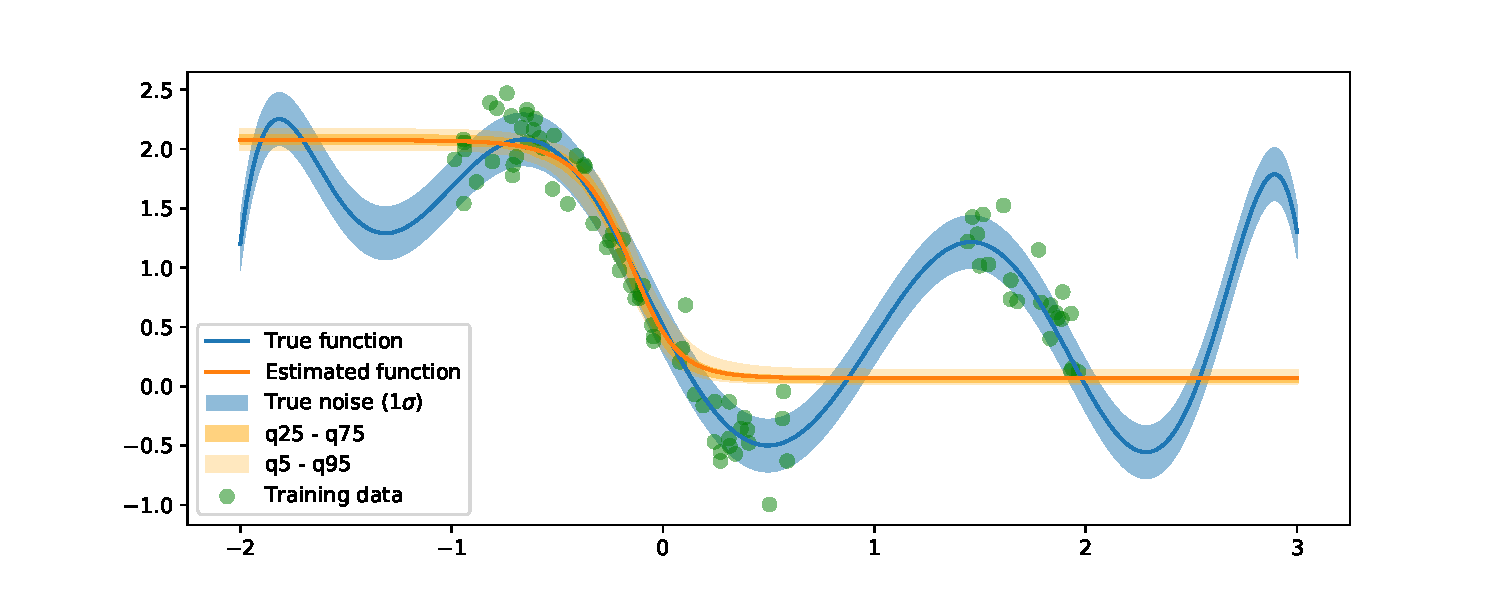
\includegraphics[width=1.0\hsize]{img/bayesian-fit-with-kl}
    \caption{
    Estimated function and the corresponding uncertainty.
    The dark-shaded region represents quantiles $q_{25}-q_{75}$, whereas the bright-shaded one represents $q_{5}-q_{95}$.
    The underlying function is not modeled well.
    The model remains stuck in this local minimum even if we increase the number of epochs from 50000 to 200000.}
    \label{fig:toy-function-whvi}
\end{figure}

Many parameter choices resulted in slow convergence and significantly underestimated uncertainty.
Our suggestions are to set $\lambda$ values that get gradually smaller as we approach the output layer and set $\sigma_0$ to be sufficiently larger than zero.
In particular, our choices for modeling the toy data set were $\lambda_1=15, \lambda_2=15,\lambda_3=0.01, \sigma_0=5$.
We also observed that the KL term in ELBO would often be much larger than the MNLL term at the beginning of the optimization.
Conversely, the MNLL term would get stuck at suboptimal value and be unable to escape this local minimum even after several thousand epochs.
After optimization, we observed several times that all but one pair of $\mu$ and $\Sigma$ parameters were almost exactly equal to zero and $\lambda$, indicating that the KL term was too dominant, drawing the variational posterior too close to the prior.

The authors also state that they obtained a model with 1541 parameters for the toy example, however we obtained one with 1537 parameters.
We were not able to identify the missing parameters and we believe that they are not hyperparameters, because the authors refer to hyperparameters separately in a Supplement section (i.e.\ not as ``parameters'').
These missing parameters might be the solution to the observed problems in our experiments.

As an attempt to improve performance, we added bias columns (to be optimized) to WHVI layers.
This addition was not enough to obtain the desired results and also introduced a considerably large number of additional parameters.
We suggest further research regarding parameter initialization.
A possible solution would be to explore hyperpriors for $\mu$ and $\rho$ to allow for greater flexibility in the sampled weights.
We found the choice of random seed not to improve results by observing the fit with seeds $5000k, k = \{1, \dots, 10\}$.
To conclude, we were not able to reproduce the uncertainty estimates, presented in the original paper.

\subsection{Regression experiments}\label{subsec:regression-experiments}
This section refers to experiments in section 3.2 and Table 3 of the original paper.
We use the experimental setup as described in section 3.2 of the original paper and section D.1 of the Supplement.
Again, the paper does not state the prior covariances $\lambda$ except for the last layer, where $\lambda = 10^{-5}$.
We choose $\lambda = 3$ for all previous layers.

The comparison between our results and the ones from the paper are presented in Table~\ref{tab:regression-experiments}.
\begin{table*}[]
    \begin{tabular}{l|llll}
               & RMSE (original) & RMSE (ours) & { }MNLL (original) & MNLL (ours) \\ \hline
    Boston     & 3.14 (0.71)     & 11.97 (0.64) & { }4.33 (1.80)     & 24188 (15730) \\
    Concrete   & 4.70 (0.72)     & 19.15 (1.21) & { }3.17 (0.37)     & 47347 (45087) \\
    Energy     & 0.58 (0.07)     & 15.54 (3.36) & { }2.00 (0.60)     & 45671 (23931) \\
    KIN8NM^*   & 0.08 (0.00)     & { }1.74 (NA) & -1.19 (0.04)       & 11343 (NA) \\
    Yacht      & 0.69 (0.16)     &              & { }1.80 (1.01)     &
    \end{tabular}
    \caption{
        WHVI regression experiments results.
        RMSE and MNLL are computed on test data sets.
        The result format is \textit{mean (std)}, where the sample mean and standard deviation are computed across 8 independent random train-test splits of the data sets.
        We used $\lambda_1=\lambda_2=15,\lambda_3=10^{-5}$ on the Boston and Concrete data sets, and $\lambda_1=\lambda_2=3,\lambda_3=10^{-5}$ for others.
        We only ran KIN8NM for one iteration that took 35 hours, however it was clear from this result and the others that the described method will not achieve the necessary results.
        For this reason, we also skipped the Naval, Power plant, and Protein data sets.
    }
    \label{tab:regression-experiments}
\end{table*}

We believe that the discrepancies are due to the missing parameters (see Subsection~\ref{subsec:toy-example}) and possibly due to different values of $\lambda$.
It is also possible that the authors invested more time into hyperparameter tuning to achieve such results, however we were unable to do the same given the considerable time and computational resources required for the experiments.
We do not evaluate WHVI performance further, because it is clear that the lack of parameters and/or the choice prior initializations are causing poor results.
